\documentclass[11pt]{article}
\usepackage[margin=1.0in]{geometry}
\usepackage{graphics,graphicx,float,subfigure,xcolor}
\usepackage{amsmath}
\usepackage{url}

\DeclareMathOperator*{\argmax}{arg\,max}
\DeclareMathOperator*{\argmin}{arg\,min}
\DeclareMathOperator{\Tr}{Tr}
\DeclareMathOperator{\sym}{sym}
\DeclareMathOperator{\lhs}{lhs}
\DeclareMathOperator{\rhs}{rhs}
\newcommand{\RNum}[1]{\uppercase\expandafter{\romannumeral #1\relax}}
\newcommand{\red}{\textcolor{red}}
\newcommand{\blue}{\textcolor{blue}}
\newcommand{\olive}{\textcolor{olive}}

\author{
  Tozoni, Davi Colli\\
  \texttt{davi.tozoni@nyu.edu}
}
\title{New Functions for Blending}

\begin{document}
\maketitle

\section{Original blending (exponential function)}
The original blending function used in the \texttt{Microstructure} package was proposed in Panetta et al.~\cite{Panetta2017}. The general idea is to merge two edges of the truss-like structure using a smooth approximation of the min function, which has the form shown below:
\begin{align}
  KS_\rho(y_1, \dots, y_n) = - \frac1\rho \ln\left(\sum_{i=1}^{n} e^{-\rho y_i} \right)
\end{align}
where the only parameter is $\rho$, which is related to the size of the blending region.

Let's take a look in the version with only two values $y_1$ and $y_2$:
\begin{align*}
  KS_\rho(y_1, y_2) &= - \frac1\rho \ln\left(e^{-\rho y_1} + e^{-\rho y_2} \right)\\
  &= - \frac1\rho \ln\left(e^{-\rho \frac{(y_1+y_2)}{2}} \left(e^{-\rho \frac{y_1 - y_2}{2}} + e^{\rho \frac{y_1-y_2}{2}} \right)\right)\\
  &= \frac{(y_1+y_2)}{2} - \frac 1\rho \ln\left(e^{-\rho \frac{y_1 - y_2}{2}} + e^{\rho \frac{y_1-y_2}{2}} \right)\\
  &= z - \frac 1\rho \ln\left(e^{-\rho \epsilon} + e^{\rho \epsilon} \right)
\end{align*}
where $z=\frac{(y_1+y_2)}{2}$ and $\epsilon=\frac{y_1 - y_2}{2}$.

Now, notice that the term $\frac 1\rho \ln\left(e^{-\rho \epsilon} + e^{\rho \epsilon} \right)$ approximates the absolute function on $\epsilon$. See Figure~\ref{fig:absolute_function}.
  \begin{figure}[!hbt]
    \begin{center}
      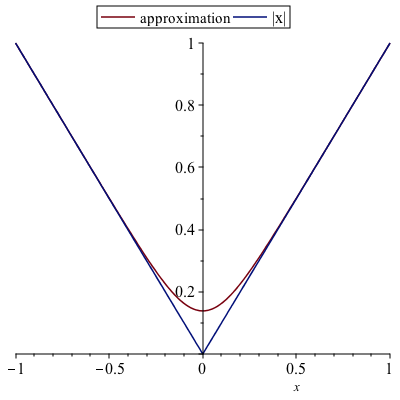
\includegraphics[width=0.5\textwidth]{absolute_function}
    \end{center}
    \caption{Comparison of absolute function and smooth version given by $\frac 1\rho \ln\left(e^{-\rho \epsilon} + e^{\rho \epsilon} \right)$.}
    \label{fig:absolute_function}
  \end{figure}

As said before, $\rho$ controls the size of the region where blending occurs. If we study the smooth absolute function, we will see that the approximating region (where result is not similar to original function) is between $-\frac2\rho$ to $\frac2\rho$. The higher the value of $\rho$, the smaller is the error between approximation and absolute value.

This indicates that we could use a different smooth approximation to the absolute value here as base for our other blending functions. Basically, each of them chooses a different way, using polynomials, to approximate the absolute function. The polynomial coefficients are then the new parameters in the shape optimization.

\section{Polynomial Blending (with monotonically increasing derivative)}
The polynomial blending idea is to create a polynomial that has the exact same behavior of the absolute function outside interval $[-\frac2\rho,\frac2\rho]$ but is smooth inside the interval. The first idea was to generate a function $f(x)$ with \textbf{monotonically increasing derivative}, to create a function that is \textbf{concave upward}.

First, let's study the derivative of the absolute function and the smooth approximation used in~\cite{Panetta2017}. See Figure~\ref{fig:derivative_absolute_function}.
  \begin{figure}[!hbt]
    \begin{center}
      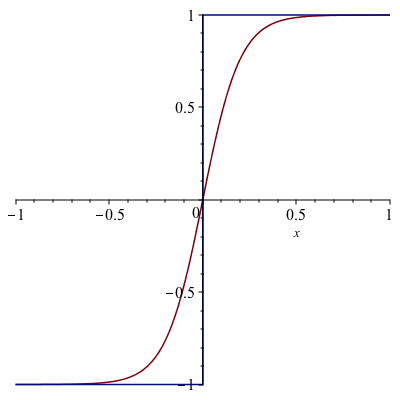
\includegraphics[width=0.5\textwidth]{derivative_absolute_function}
    \end{center}
    \caption{Comparison of derivative of absolute function and smooth version given by $\frac 1\rho \ln\left(e^{-\rho \epsilon} + e^{\rho \epsilon} \right)$.}
    \label{fig:derivative_absolute_function}
  \end{figure}

Now, notice that, to achieve our objective, we need a derivative that has positive slope during the whole approximation interval and which has derivative equal to $0$ on both ends of the blending region. This defines the properties we want for the second derivative of the $f(x)$, called here $r(x)$. An example of a valid $r(x)$ is shown in Figure~\ref{fig:positive_function}.
  \begin{figure}[!hbt]
    \begin{center}
      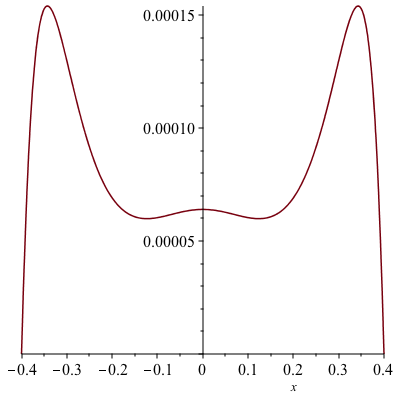
\includegraphics[width=0.5\textwidth]{positive_function}
    \end{center}
    \caption{Example of function $r(x)$, representing second derivative of $f(x)$.}
    \label{fig:positive_function}
  \end{figure}
  
But how to construct function $f(x)$ based on this. Let's work on the opposite direction. First, let's create function $r(x)$ corresponding to the second derivative. To make sure it is always positive and $0$ at $-\frac2\rho$ and $\frac2\rho$ we proposed the following:
\begin{align}
  r(x) = -\left(a_0 + a_2 x^2 + a_4 x^4 \dots + a_{2n} x^{2n}  \right)^2 \left(x + \frac2\rho\right) \left(x - \frac2\rho\right)
\end{align}
where $a_{2*(i-1)}$ corresponds to the $i$th parameter for blending (outside $\rho$). Notice that we removed the odd coefficients in order to make sure the function has reflectional symmetric with respect to the $y$ axis.

Then, we build $h(x)$ by integrating $r(x)$, starting from $-\frac{2}\rho$:
\begin{align*}
  h(x) = \int_{-2/\rho}^{x} r(z) dz
\end{align*}
and we then normalize this integral so that it can be between $-1$ and $1$, obtaining the slope function $g(x)$.
\begin{align*}
  g(x) = 2 \frac{h(x)}{h(2/\rho)} - 1
\end{align*}
  
Again, to obtain now our smooth absolute function, we do the same thing, integrating $g(x)$:
\begin{align*}
  q(x) = \int_{-2/\rho}^{x} g(z) dz
\end{align*}
but we need to make sure that $f(2/\rho) = 2/\rho$. To obtain this, we need an offset $a$ on $q(x)$ such that $f(2/\rho) = q(2/\rho) + a = 2/\rho$. So, $a = 2/\rho - q(2/\rho)$. And, finally,
\begin{align*}
  f(x) = q(x) - 2/\rho - q(2/\rho)
\end{align*}

An example of the final $f(x)$ is shown in Figure~\ref{fig:example_f1}.
  \begin{figure}[!hbt]
    \begin{center}
      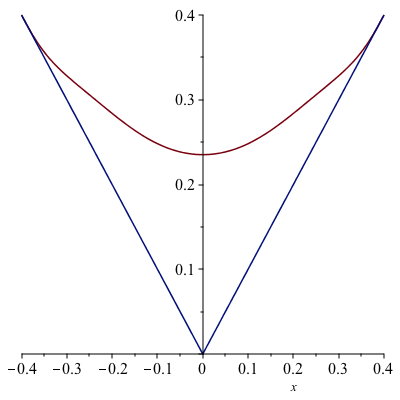
\includegraphics[width=0.5\textwidth]{example_f1}
    \end{center}
    \caption{Example of function $f(x)$ with monotonically increasing derivative, generating convex blending shape.}
    \label{fig:example_f1}
  \end{figure}


To understand better the functions and to plot examples, please take a look on Maple script\linebreak \path{KS_monotonic_derivative_8parameters.mw}.

\section{Non-convex Polynomial Blending}
After experiments, we noticed that in some cases it seemed important to have blending regions that are not always convex. To obtain this effect, we simply removed power of $2$ from the first polynomial term in $r(x)$, obtaining:
 \begin{align}
  r(x) = -\left(a_0 + a_2 x^2 + a_4 x^4 \dots + a_{2n} x^{2n}  \right) \left(x + \frac2\rho\right) \left(x - \frac2\rho\right)
\end{align}

The rest of the steps to obtain $f(x)$ are exactly the same as before. An example is shown in Figure~\ref{fig:example_f2}. To find more information, please refer to script \path{KS_nonconvex_8parameters.mw}.
  \begin{figure}[!hbt]
    \begin{center}
      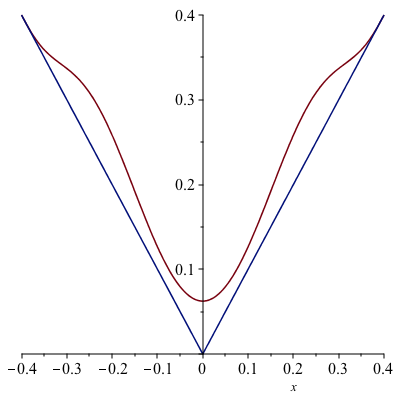
\includegraphics[width=0.5\textwidth]{example_f2}
    \end{center}
    \caption{Example of function $f(x)$ which can generate non-convex shapes on blending regions.}
    \label{fig:example_f2}
  \end{figure}

\section{Piecewise Polynomial Blending}
The third blending function implemented corresponds to a piecewise polynomial function. The idea is to define the curvature of $f'(x)$ on each piece of the blending region. Notice that, because we are working with symmetric functions, we can define these curvatures only on the left side, for example, as shown in Figure~\ref{fig:curvatures} and then reflect it (with respect to $y$ axis) on positive $x$ values.
  \begin{figure*}[!hbt]
    \centering
    \begin{subfigure}
      \centering
      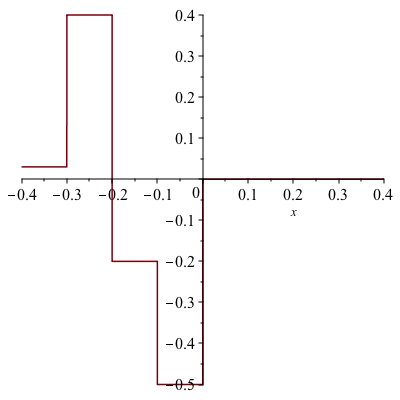
\includegraphics[width=0.4\linewidth]{curvatures}
    \end{subfigure}%
    \begin{subfigure}
      \centering
      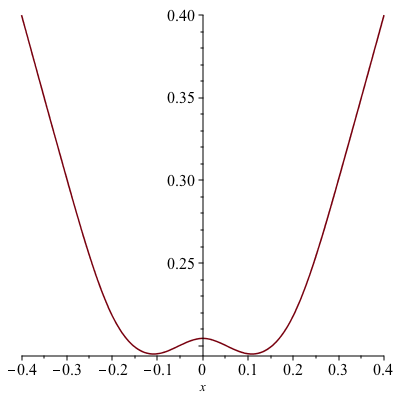
\includegraphics[width=.4\linewidth]{curvatures_result}
    \end{subfigure}
    \caption{Example of curvatures chosen and corresponding result.}
    \label{fig:curvatures}
  \end{figure*}

Then, we work in a similar way as before. First we integrate the curvature function $w(x)$:
\begin{align*}
  r(x) = \int_{-2/\rho}^{x} w(z) dz
\end{align*}

Then, we integrate again to obtain the curve $h(x)$:
\begin{align*}
  h(x) = \int_{-2/\rho}^{x} r(z) dz
\end{align*}

After this, we normalize to obtain values from $-1$ to $1$. See also Figure~\ref{fig:piecewise_slope}.
\begin{align*}
  g(x) = \frac{h(x)}{h(0)} - 1
\end{align*}

  \begin{figure}[!hbt]
    \begin{center}
      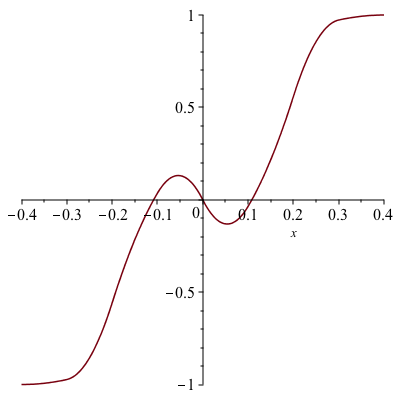
\includegraphics[width=0.5\textwidth]{piecewise_slope}
    \end{center}
    \caption{Function $g(x)$ representing slope of the final piecewise function.}
    \label{fig:piecewise_slope}
  \end{figure}

Finally, we integrate one last time and normalize the result obtaining:
\begin{align*}
  q(x) = \int_{-2/\rho}^{x} g(z) dz\\
  f(x) = q(x) + 2/\rho - q(2/\rho)
\end{align*}

The result can be seen in Figure~\ref{fig:example_fpiecewise}. For more information, please take a look at script \path{KS_piecewise.mw} (which presents the recursive definition of this blending function used in the implementation) and \path{KS_piecewise_example.mw} (which presents an example with 4 pieces and the functions as described here).

 \begin{figure}[!hbt]
    \begin{center}
      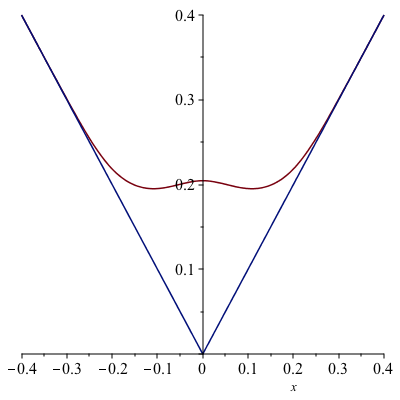
\includegraphics[width=0.5\textwidth]{example_fpiecewise}
    \end{center}
    \caption{Example of a piecewise function $f(x)$, approximating $|x|$ smoothly.}
    \label{fig:example_fpiecewise}
  \end{figure}

\section{Approximating the minimum of more than two numbers}
In the case of more than 2 values, it becomes more difficult to apply the approximation of the absolute function directly as presented before. However, we know the following:
\[
\min(y_1, y_2, y_3, \dots, y_n) = 
\begin{cases} 
      \min(\min(y_1, y_2, \dots, y_{n-1}), y_n) & n > 2 \\
      \min(y_1, y_2) & n = 2 
   \end{cases}
\]

We need to be cautious here because the smooth approximation of $\min$ will not be symmetric in terms of the order of the arguments. For example, $\min(1,2,3)$ may be different from $\min(3,2,1)$, depending on the approximation. That said, we can use the symmetric version shown below:
\[
\min(y_1, y_2, y_3, \dots, y_n) = 
\begin{cases} 
      \frac1n\sum_{i=1}^n\min(y_i, \min(y_1, \dots, y_{i-1}, y_{i+1}, \dots, y_{n})) & n > 2 \\
      \min(y_1, y_2) & n = 2 
   \end{cases}
\]

Notice that we can implement this function in a recursive way. Now, we can simply use one of the 3 blending functions described above for each $\min$ call between two numbers. Also, notice that the approximations are propagated and, at the last level calls, you will not have the $\min$ operation between the original numbers. To avoid having high accumulation of these \emph{errors}, at each recursive call the parameter related to blending region $s = 1/\rho$ is divided by a scalar $\alpha > 1$. So, if $\text{smin}_\rho()$ is our smooth minimum function with parameter $\rho$, we have:
 \[
\text{smin}_\rho(y_1, y_2, y_3, \dots, y_n) = 
\begin{cases} 
      \frac1n\sum_{i=1}^n\text{smin}_\rho(y_i, \text{smin}_{\rho*\alpha}(y_1, \dots, y_{i-1}, y_{i+1}, \dots, y_{n})) & n > 2 \\
      \text{smin}_\rho(y_1, y_2) & n = 2 
   \end{cases}
\]

\bibliographystyle{abbrv}
\bibliography{blending} 

\end{document}
